\documentclass[tikz,border=6pt]{standalone}
\usepackage{amsmath,amssymb,mathtools,physics,bm,nicefrac,wasysym}
\usepackage{xcolor}

\definecolor{colone}{RGB}{180,60,60}
\definecolor{coltwo}{RGB}{60,110,180}
\definecolor{colthree}{RGB}{60,140,80}

\definecolor{accent}{HTML}{A13D2C}
\definecolor{accent2}{HTML}{2B5F6B}
\definecolor{muted}{HTML}{5A564F}
\definecolor{panel}{HTML}{F8F6F0}
\definecolor{linecol}{HTML}{D8D2C4}
\definecolor{ink}{HTML}{1E1C1A}
\definecolor{astroblue}{HTML}{1B4F72}
\definecolor{astrodark}{HTML}{17202A}
\definecolor{sunyellow}{HTML}{E8A33D}

\usetikzlibrary{calc,arrows.meta,positioning,decorations.pathreplacing,decorations.markings,angles,quotes,shapes.geometric}
\usepackage{tikz-3dplot}

\newcommand{\vecr}{\vec r}
\newcommand{\vecL}{\vec L}
\newcommand{\vecA}{\vec A}
\newcommand{\vecf}{\vec f}
\newcommand{\vecF}{\vec F}
\newcommand{\vecp}{\vec p}
\newcommand{\avg}[1]{\left\langle #1\right\rangle}
\newcommand{\vecx}{\vec x}
\newcommand{\hatn}{\hat n}
\newcommand{\rhat}{\hat r}
\newcommand{\phihat}{\hat\phi}
\newcommand{\thetahat}{\hat\theta}
\newcommand{\note}[1]{\textcolor{blue!60!black}{\textit{[#1]}}}

% Astronomical acronyms
\newcommand{\LST}{\mathrm{LST}}
\newcommand{\GST}{\mathrm{GST}}
\newcommand{\GMST}{\mathrm{GMST}}
\newcommand{\GAST}{\mathrm{GAST}}
\newcommand{\LMST}{\mathrm{LMST}}
\newcommand{\LAST}{\mathrm{LAST}}
\newcommand{\UT}{\mathrm{UT}}
\newcommand{\UTC}{\mathrm{UTC}}
\newcommand{\TAI}{\mathrm{TAI}}
\newcommand{\TT}{\mathrm{TT}}
\newcommand{\TDB}{\mathrm{TDB}}
\newcommand{\JD}{\mathrm{JD}}
\newcommand{\MJD}{\mathrm{MJD}}
\newcommand{\EoT}{\mathrm{EoT}}
\newcommand{\SNR}{\mathrm{SNR}}
\newcommand{\RON}{\mathrm{RON}}

% Helper commands for specific diagrams
\newcommand{\midlinelabel}[3]{
    \node (midlabel) at ($ (#1)!.5!(#2) $) {#3};
    \draw[stealth-] (#1) --  (midlabel);
    \draw[-stealth] (midlabel) -- (#2);
}
\newcommand{\midlinelabell}[3]{
    \node[fill = white, inner sep = 0.2pt, outer sep=3pt] (midlabel) at ($ (#1)!.5!(#2) $) {#3};
    \draw[stealth-] (#1) --  (midlabel);
    \draw[-stealth] (midlabel) -- (#2);
}
\newcommand{\midlinelabelll}[3]{
    \node[fill = white, inner sep = 0.2pt, outer sep=3pt,scale=0.6] (midlabel) at ($ (#1)!.5!(#2) $) {#3};
    \draw[stealth-] (#1) --  (midlabel);
    \draw[-stealth] (midlabel) -- (#2);
}



\begin{document}
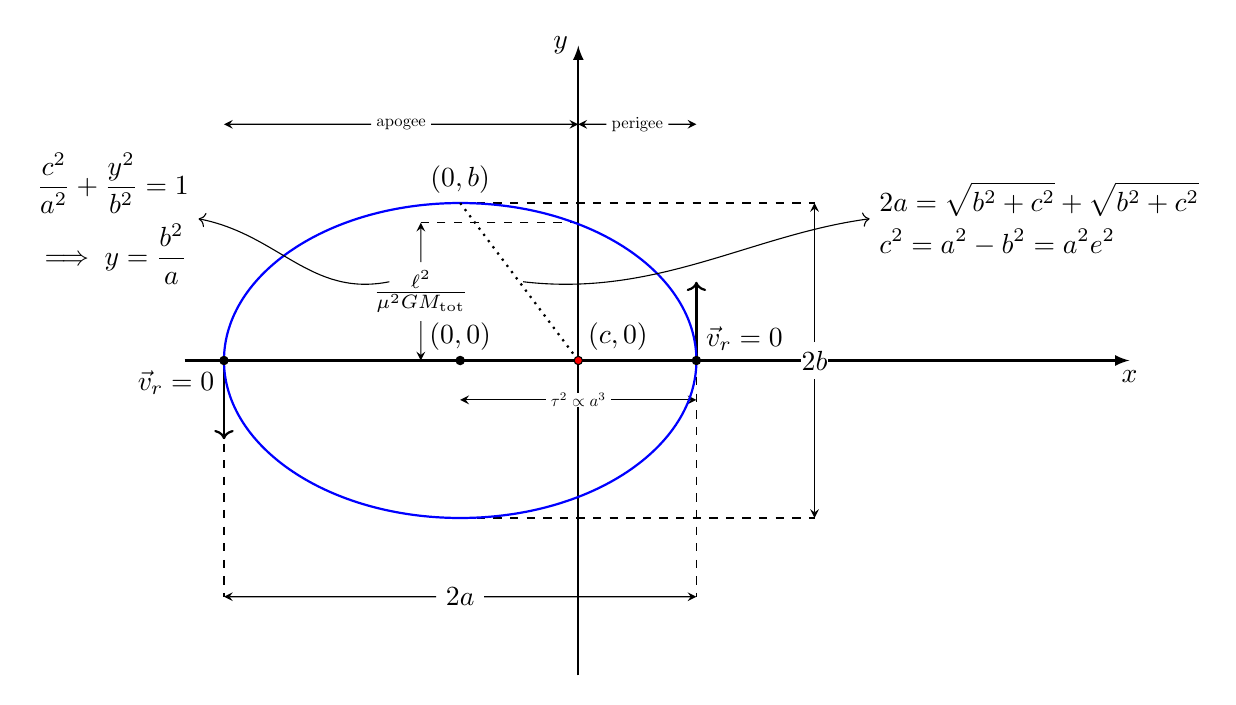
\begin{tikzpicture}
			% Axis
			\draw[-latex, thick] (5,0) -- (5,8) node[left] {$y$};
			\draw[-latex, thick] (0,4) -- (12,4) node[below] {$x$};
			\midlinelabell{3,4}{3,5.75}{$\frac{\ell^2}{\mu^2GM_{\rm tot}}$};
			
			% Key points
			\coordinate (F) at (5,4);       % illustrative focus = (c,0)
			\coordinate (Top) at (3.5,6);   % illustrative top point = (0,b)
			
			% Lines
			\draw[dashed] (5,5.75) -- (3,5.75);
			\draw[dashed] (0.5,4) -- (0.5,1);
			\draw[dashed] (6.5,4) -- (6.5,1);
			\draw[->,thick] (6.5,4)--(6.5,5);
			\draw[->,thick] (0.5,4)--(0.5,3);
			\draw[dashed] (3.5,2) -- (8,2);
			\draw[dashed] (3.5,6) -- (8,6);
			
			%% Labels
			\midlinelabel{0.5,1}{6.5,1}{$2a$}
			\midlinelabelll{3.5,3.5}{6.5,3.5}{$\tau^2\propto a^3$}
			\midlinelabell{8,2}{8,6}{$2b$}
			\midlinelabelll{6.5,7}{5,7}{perigee}
			\midlinelabelll{0.5,7}{5,7}{apogee}
			
			% Ellipse
			\draw[blue, thick] (3.5,4) circle [x radius = 3, y radius = 2];
			
			% Dotted line from (0,b) to (c,0)
			\draw[dotted, thick] (Top) -- (F);
			
			% Points
			\draw[fill=black] (3.5,4) circle [radius=1.5pt] node[above] {$(0,0)$};
			\draw[fill=black] (0.5,4) circle [radius=1.5pt] node[below left] {$\vec{v}_{r}=0$};
			\draw[fill=black] (6.5,4) circle [radius=1.5pt] node[above right] {$\vec{v}_{r}=0$};
			\draw[fill=red] (F) circle [radius=1.5pt] node[above right] {$(c,0)$};
			\node[above] at (Top)  {$(0,b)$};
			
			% Calculation on right
			\node[anchor=west, align=left] (calcbox) at (8.7,5.8) {
				$\displaystyle 2a=\sqrt{b^2+c^2}+\sqrt{b^2+c^2}$ \\[3pt]
				$\displaystyle c^2=a^2-b^2=a^2e^2$
			};
			\node[anchor=west, align=left] (calcbox2) at (-2,5.8) {
				$\displaystyle \frac{c^2}{a^2}+\frac{y^2}{b^2}=1$ \\[3pt]
				$\displaystyle \implies y=\frac{b^2}{a}$ 
			};
			% Squiggly arrow from focus to calculation
			\draw[->, thin]
			(4.3,5).. controls (6.0,4.8) and (7.2,5.6) ..
			(calcbox.west);
			\draw[->, thin]
			(2.6,5).. controls (1.6,4.8) and (1.2,5.6) ..
			(calcbox2.east);
		\end{tikzpicture}
\end{document}
